\begin{frame}
\frametitle{Problem Statement-Quadrilateral Exercise}
\begin{enumerate}[label=(\roman*)]
\item The side AB of a parallelogram ABCD is produced to any point P. A line through A and
parallel to CP meets CB produced at Q and then parallelogram PBQR is completed. Show
that ar(ABCD) = ar(PBQR).
\textbf{Soln:}\\
Given:- CP $\parallel$ AQ
  \end{enumerate} 
\url{https://github.com/Rajolep/_Geometry/blob/master/codes/quadr/quadexer.py}
\begin{figure}
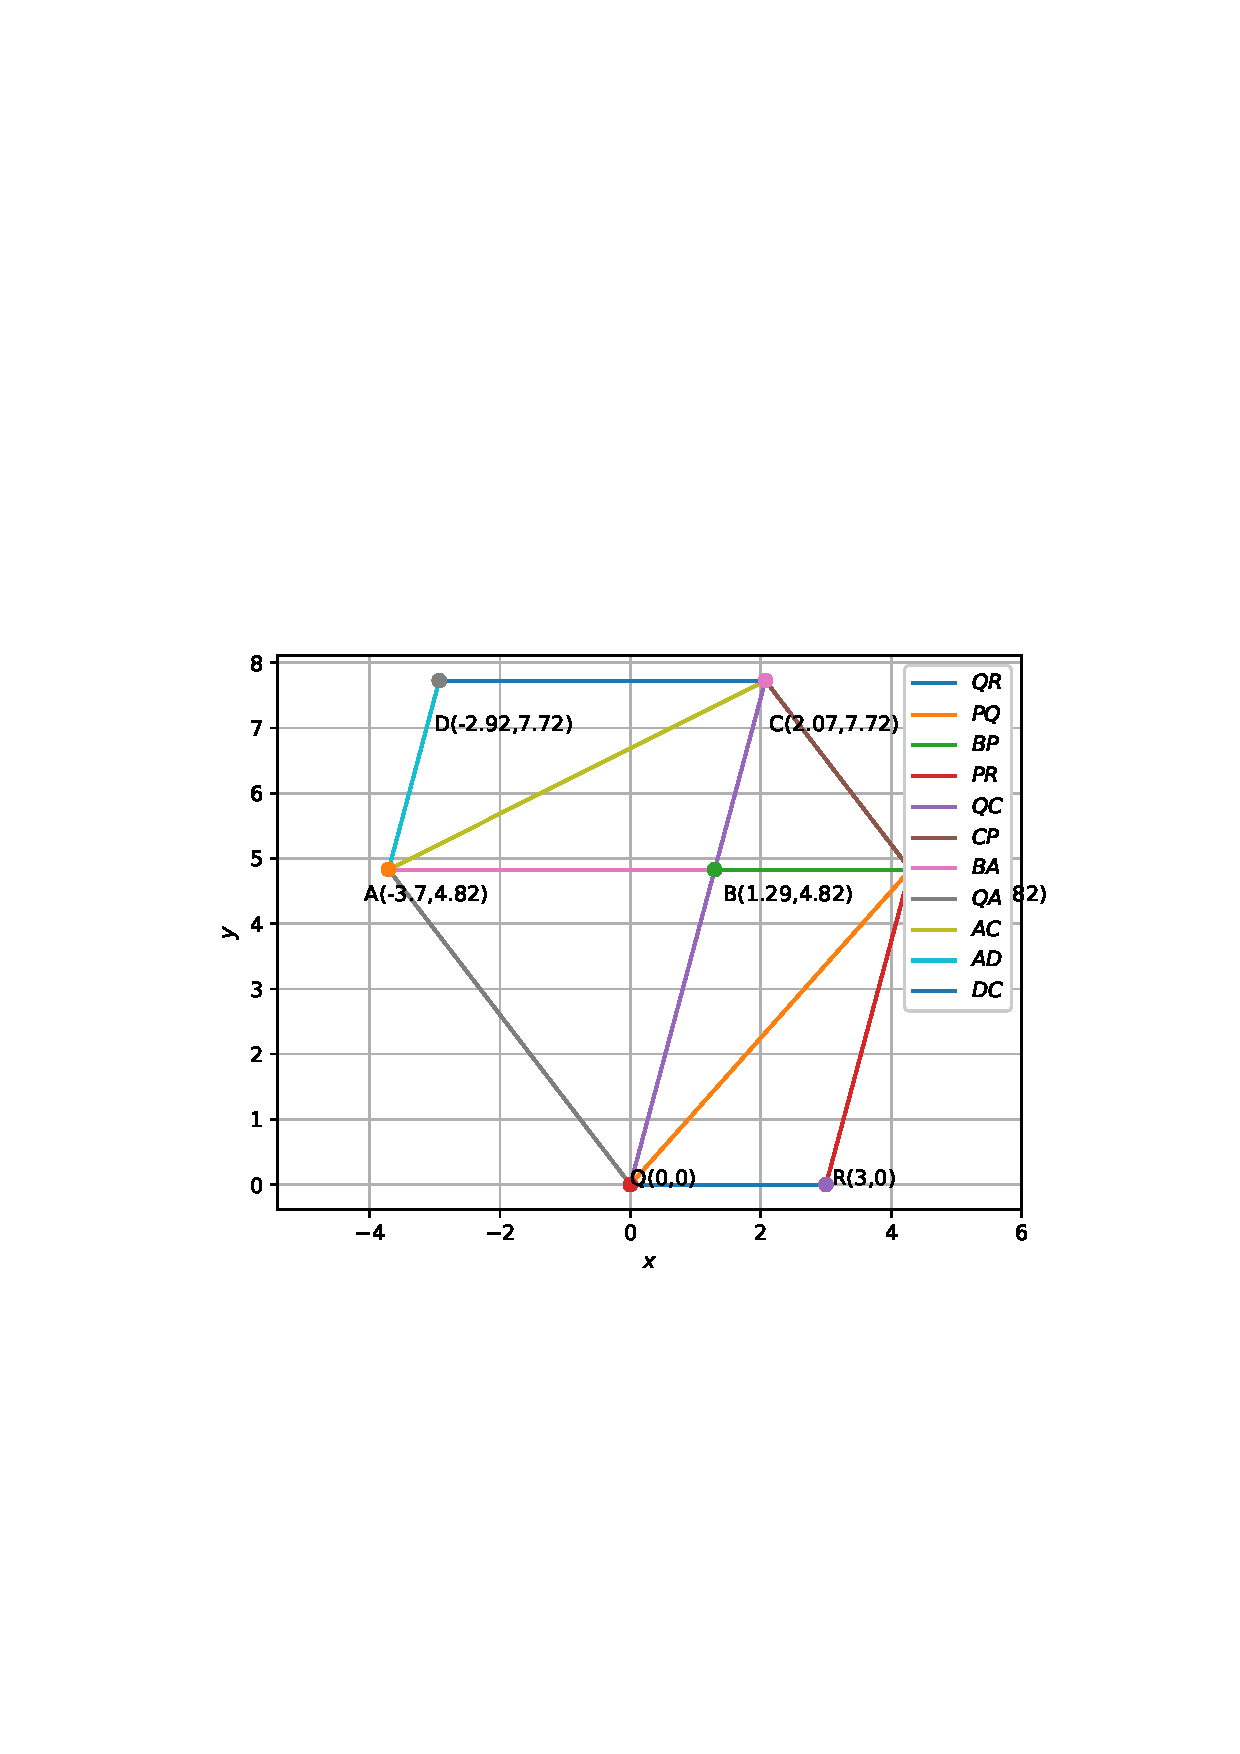
\includegraphics[scale=0.3]{./figs/quadexer.png}
\end{figure}
\end{frame}
\begin{frame}
\begin{figure}
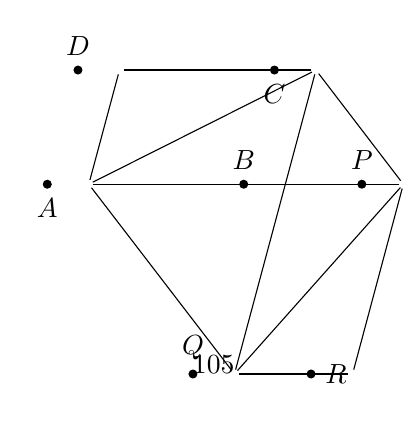
\begin{tikzpicture}
[scale =0.5,>=stealth,point/.style = {draw, circle, fill = black, inner sep = 1pt},]
\node (D) at (-2.92,7.72)[point,label=above :$D$] {};
\node (C) at (2.07,7.72)[point,label=below :$C$] {};
\node (A) at (-3.70,4.82)[point,label=below :$A$] {};
\node (B) at (1.29,4.82)[point,label=above :$B$] {};
\node (P) at (4.29,4.82)[point,label=above :$P$] {};
\node (Q) at (0,0)[point,label=above :$Q$] {};
\node (R) at (3,0)[point,label=right :$R$] {};
\tkzMarkAngle[fill=red!105,size=.4,mark=](C,R,Q)
\tkzLabelAngle[pos=0.75](C,R,Q){$105\degree$}

\draw (A)--(P);
\draw (C)--(P);
\draw (Q)--(C);
\draw (C)--(D);
\draw (D)--(A);
\draw (P)--(R);
\draw (C)--(A);
\draw (P)--(Q);

\draw (R)--(Q);
\draw (A)--(Q);
\end{tikzpicture}

\end{figure}
\url{https://github.com/Rajolep/_Geometry/blob/master/figs/quadexe.tex}
\end{frame}
\begin{frame}
\begin{align*}
CP \parallel AQ\\
\end{align*}
area of $\triangle{ACQ}$ =  area of $\triangle{AQP}$\\
subtract area$\triangle{ABQ}$ in above Eqn\\
ar$\triangle{ACQ}$-ar$\triangle{ABQ}$ = ar$\triangle{APQ}$-ar$\triangle{ACQ}$\\
ar$\triangle{ABC}$ = ar$\triangle{PBQ}$....(1)\\
$\triangle{ABC} \cong \triangle{ADC}$\\
ar$\triangle{ABC}$ = ar$\triangle{ADC}$\\
ar$\triangle{ABC}$ = ar$\triangle{ADC}$ = $\frac{1}{2}(ABCD)$...(2)\\
\end{frame}
\begin{frame}
similarly in PBQR,\\
$\triangle{PBQ} \cong \triangle{PRQ}$\\
ar$\triangle{PBQ}$ = ar$\triangle{PRQ}$\\
ar$\triangle{PBQ}$ = ar$\triangle{PRQ}$ = $\frac{1}{2}(ABCD)$....(3)\\
frm (1)\\
$\triangle{ABC}$ = $\triangle{PBQ}$\\
frm (2)  (3)\\
$\frac{1}{2}(ABCD)$ = $\frac{1}{2}(ABCD)$\\
Ar(ABCD) = Ar(PBQR)\\
\end{frame}